\begin{figure}[!htb]
	\centering

	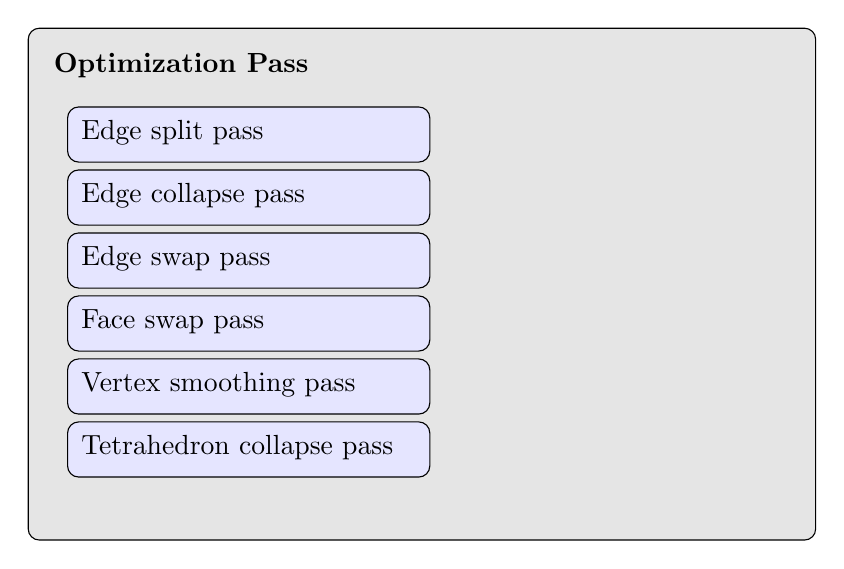
\begin{tikzpicture}

		\draw[rounded corners, fill=black!10] (0, 0) rectangle (10, 6.5);
		\node[anchor=north west,font=\bfseries, xshift=0.2cm, yshift=-0.2cm] at (0,6.5) {Optimization Pass};
		\draw[rounded corners, fill=blue!10] (0.5, 4.8) rectangle (5.1, 5.5);
		\node[anchor=north west, xshift=0.05cm, yshift=-0.05cm] at (0.5,5.5) {Edge split pass};
		\draw[rounded corners, fill=blue!10] (0.5, 4) rectangle (5.1, 4.7);
		\node[anchor=north west, xshift=0.05cm, yshift=-0.05cm] at (0.5,4.7) {Edge collapse pass};
		\draw[rounded corners, fill=blue!10] (0.5, 3.2) rectangle (5.1, 3.9);
		\node[anchor=north west, xshift=0.05cm, yshift=-0.05cm] at (0.5,3.9) {Edge swap pass};
		\draw[rounded corners, fill=blue!10] (0.5, 2.4) rectangle (5.1, 3.1);
		\node[anchor=north west, xshift=0.05cm, yshift=-0.05cm] at (0.5,3.1) {Face swap pass};
		\draw[rounded corners, fill=blue!10] (0.5, 1.6) rectangle (5.1, 2.3);
		\node[anchor=north west, xshift=0.05cm, yshift=-0.05cm] at (0.5,2.3) {Vertex smoothing pass};
		\draw[rounded corners, fill=blue!10] (0.5, 0.8) rectangle (5.1, 1.5);
		\node[anchor=north west, xshift=0.05cm, yshift=-0.05cm] at (0.5,1.5) {Tetrahedron collapse pass};

	\end{tikzpicture}

	\caption{Optimization process scheme}\label{fig:optimizationPass}
\end{figure}
